\documentclass[12pt, a4paper]{article}

% Packages
\usepackage[utf8]{inputenc}
\usepackage[T1]{fontenc}
\usepackage{lmodern}
\usepackage[left=2.5cm, right=2.5cm, top=3cm, bottom=3cm]{geometry}
\usepackage{graphicx}
\usepackage{booktabs}
\usepackage{array}
\usepackage{tabularx}
\usepackage{amsmath}
\usepackage{hyperref}
\usepackage{enumitem}
\usepackage{float}
\usepackage{caption}
\usepackage{setspace}
\usepackage{parskip}
\usepackage{fancyhdr}
\usepackage{titlesec}
\usepackage{xcolor}
\usepackage{listings}
\usepackage{url}
\usepackage{tikz}
\usepackage{multirow}
\usepackage{colortbl}
\usetikzlibrary{shapes.geometric, arrows.meta, positioning, calc}

% Colours
\definecolor{solarblue}{RGB}{31, 78, 121}
\definecolor{solaramber}{RGB}{180, 100, 20}
\definecolor{solargray}{RGB}{80, 80, 80}
\definecolor{lightgray}{RGB}{245, 245, 245}
\definecolor{codebg}{RGB}{248, 248, 248}

% Section formatting
\titleformat{\section}{\large\bfseries\color{solarblue}}{}{0em}{\thesection\quad}[\titlerule]
\titleformat{\subsection}{\normalsize\bfseries\color{solaramber}}{}{0em}{\thesubsection\quad}
\titleformat{\subsubsection}{\normalsize\itshape\color{solargray}}{}{0em}{\thesubsubsection\quad}

% Hyperref config
\hypersetup{
    colorlinks=true,
    linkcolor=solarblue,
    urlcolor=solaramber,
    citecolor=solarblue
}

% Header/Footer
\pagestyle{fancy}
\fancyhf{}
\fancyhead[L]{\small\textit{SolarIntel}}
\fancyhead[R]{\small\textit{Solar Energy Generation Prediction}}
\fancyfoot[C]{\thepage}
\renewcommand{\headrulewidth}{0.4pt}

% Code listing style
\lstset{
    basicstyle=\ttfamily\small,
    backgroundcolor=\color{codebg},
    frame=single,
    rulecolor=\color{solarblue!30},
    breaklines=true,
    columns=fullflexible,
    keepspaces=true,
    keywordstyle=\color{solarblue}\bfseries,
    commentstyle=\color{solargray}\itshape,
    stringstyle=\color{solaramber}
}

% Spacing
\onehalfspacing
\setlength{\parindent}{0pt}

% Title Page
\begin{document}

\begin{titlepage}
    \centering
    \vspace*{1.5cm}

    {\huge\bfseries\color{solarblue} SolarIntel}\\[0.6cm]
    {\Large\color{solaramber} Solar Energy Generation Prediction}\\[0.3cm]
    {\large Using EMHIRES and NASA POWER Data}\\[0.4cm]
    \rule{\linewidth}{1.5pt}\\[0.8cm]

    {\large\textbf{Project Report}}

    \vspace{1.5cm}

    \begin{tabular}{rl}
        \textbf{Live Demo:} & \url{https://huggingface.co/spaces/priyanshutomar2024/SolarIntel} \\[4pt]
        \textbf{Domain:} & Machine Learning, Renewable Energy \\[4pt]
        \textbf{Models:} & Linear Regression, Random Forest Regressor \\[4pt]
        \textbf{Deployment:} & Streamlit on Hugging Face Spaces \\[4pt]
        \textbf{Coverage:} & 29 European Countries, 2001--2015, Hourly \\
    \end{tabular}

    \vspace{2cm}

    \vfill
    {\large \today}
\end{titlepage}

% Table of Contents
\newpage
{\singlespacing
\tableofcontents
}
\newpage

% Abstract
\begin{abstract}
\noindent
Accurate forecasting of solar energy generation is essential for grid balancing, energy market operations, and renewable infrastructure planning across Europe. This report presents \textbf{SolarIntel}, an end-to-end machine learning system that predicts hourly solar capacity factors for 29 European countries by fusing 15 years of photovoltaic generation data from the European Commission's EMHIRES dataset with satellite-derived meteorological observations from NASA's POWER API. The resulting dataset comprises approximately 3.8 million hourly records and 34 features. Two regression models are trained and evaluated: a Linear Regression baseline ($R^2 = 0.788$) and a Random Forest Regressor ($R^2 = 0.911$). The superior model is deployed through an interactive Streamlit web application hosted on Hugging Face Spaces, enabling real-time prediction, 24-hour generation profiling, and cross-country comparison.
\end{abstract}

\newpage

% Section 1
\section{Introduction}

Solar energy is one of the fastest-growing renewable energy sources globally. Accurate forecasting of solar energy generation is critical for grid stability, energy trading, and infrastructure planning. The variability of solar output, driven by weather conditions, geographic location, and time of day, makes prediction a non-trivial challenge.

This project, \textbf{SolarIntel}, addresses this challenge by building an end-to-end machine learning pipeline that predicts hourly solar energy capacity factors across 29 European countries. The system fuses 15 years of solar generation data from the European Commission's EMHIRES dataset with hourly meteorological observations from NASA's POWER API. Two regression models are trained, evaluated, and compared. The best-performing model is deployed through an interactive Streamlit web application hosted on Hugging Face Spaces.

\subsection{Objectives}

\begin{itemize}[noitemsep]
    \item Collect, clean, and merge solar generation and weather datasets spanning 2001--2015.
    \item Engineer temporal and geographic features suitable for regression modelling.
    \item Train and evaluate two regression models: Linear Regression and Random Forest Regressor.
    \item Deploy the trained model as an interactive web application for real-time predictions.
\end{itemize}

\subsection{Scope}

The pipeline covers 29 European countries at hourly resolution. The target variable is Capacity Factor, a normalised measure of solar output ranging from 0.0 (no generation) to 1.0 (maximum rated output). The final dataset contains approximately 3.8 million rows and 34 features.

% Section 2
\newpage
\section{Data Sources}

Two primary datasets are used. Both are publicly available.

\subsection{EMHIRES PV Dataset}

The European Meteorological-derived High-resolution RES generation time series for present and future scenarios (EMHIRES) dataset is published by the European Commission's Joint Research Centre (JRC). The PV module provides hourly solar capacity factors for European countries from 1986 to 2015.

\begin{table}[H]
    \centering
    \caption{EMHIRES PV Dataset Summary}
    \begin{tabular}{ll}
        \toprule
        \textbf{Attribute} & \textbf{Detail} \\
        \midrule
        Source & European Commission, JRC \\
        Temporal Coverage & 1986--2015 (hourly) \\
        Spatial Coverage & 29 European countries \\
        Format & Wide-format CSV (countries as columns) \\
        Target Variable & Capacity Factor (0.0--1.0) \\
        \bottomrule
    \end{tabular}
\end{table}

The dataset is in wide format with each column representing a country code (e.g., AT for Austria, ES for Spain). Each row corresponds to one hour. The data was filtered to the 2001--2015 range to align with the availability of NASA weather data.

\subsection{NASA POWER API}

The Prediction Of Worldwide Energy Resources (POWER) project by NASA provides satellite-derived meteorological data. Hourly observations were fetched via the POWER API for all 29 EMHIRES countries using geographic centroids.

\begin{table}[H]
    \centering
    \caption{NASA POWER Weather Parameters}
    \begin{tabular}{lll}
        \toprule
        \textbf{API Parameter} & \textbf{Renamed To} & \textbf{Unit} \\
        \midrule
        ALLSKY\_SFC\_SW\_DWN & Irradiance & W/m\textsuperscript{2} \\
        T2M & Temperature & \textdegree C \\
        WS2M & Wind Speed & m/s \\
        \bottomrule
    \end{tabular}
\end{table}

Data was collected for each country and each year (2001--2015) individually, with a 0.5-second delay between requests to respect API rate limits. The full fetch takes approximately 20 minutes due to the volume of requests (29 countries $\times$ 15 years = 435 API calls).

% Section 3
\newpage
\section{Data Pipeline}

The pipeline follows a sequential flow: data loading, cleaning, transformation, merging, encoding, and export. Each stage is implemented as a standalone Python module and also consolidated in a single end-to-end script. Figure~\ref{fig:pipeline} illustrates the full architecture.

\begin{figure}[H]
\centering
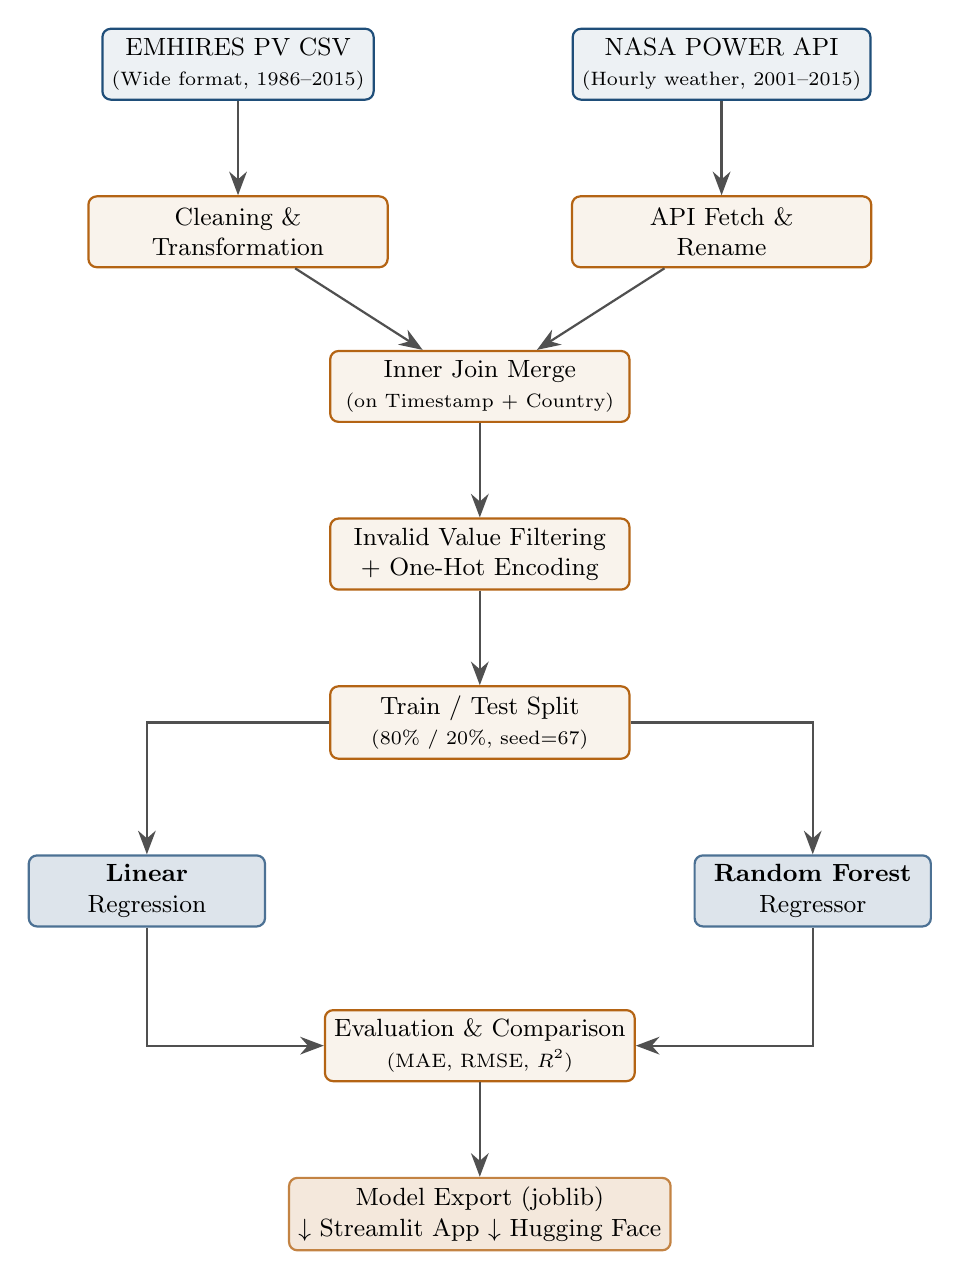
\begin{tikzpicture}[
    node distance=1.2cm and 2.5cm,
    every node/.style={font=\small},
    databox/.style={rectangle, draw=solarblue, fill=solarblue!8, rounded corners=3pt, minimum width=3.2cm, minimum height=0.9cm, align=center, thick},
    procbox/.style={rectangle, draw=solaramber, fill=solaramber!8, rounded corners=3pt, minimum width=3.8cm, minimum height=0.9cm, align=center, thick},
    modelbox/.style={rectangle, draw=solarblue!80, fill=solarblue!15, rounded corners=3pt, minimum width=3cm, minimum height=0.9cm, align=center, thick},
    deploybox/.style={rectangle, draw=solaramber!80, fill=solaramber!15, rounded corners=3pt, minimum width=4cm, minimum height=0.9cm, align=center, thick},
    arrow/.style={-{Stealth[length=3mm]}, thick, color=solargray}
]

% Data sources
\node[databox] (emhires) {EMHIRES PV CSV\\{\scriptsize (Wide format, 1986--2015)}};
\node[databox, right=of emhires] (nasa) {NASA POWER API\\{\scriptsize (Hourly weather, 2001--2015)}};

% Processing
\node[procbox, below=of emhires] (clean) {Cleaning \&\\Transformation};
\node[procbox, below=of nasa] (fetch) {API Fetch \&\\Rename};

% Merge
\node[procbox, below=1.5cm of $(clean)!0.5!(fetch)$] (merge) {Inner Join Merge\\{\scriptsize (on Timestamp + Country)}};

% Filter + Encode
\node[procbox, below=of merge] (filter) {Invalid Value Filtering\\+ One-Hot Encoding};

% Split
\node[procbox, below=of filter] (split) {Train / Test Split\\{\scriptsize (80\% / 20\%, seed=67)}};

% Models
\node[modelbox, below left=1.2cm and 0.8cm of split] (lr) {\textbf{Linear}\\Regression};
\node[modelbox, below right=1.2cm and 0.8cm of split] (rfr) {\textbf{Random Forest}\\Regressor};

% Evaluation
\node[procbox, below=1.5cm of $(lr)!0.5!(rfr)$] (eval) {Evaluation \& Comparison\\{\scriptsize (MAE, RMSE, $R^2$)}};

% Export + Deploy
\node[deploybox, below=of eval] (deploy) {Model Export (joblib)\\$\downarrow$ Streamlit App $\downarrow$ Hugging Face};

% Arrows
\draw[arrow] (emhires) -- (clean);
\draw[arrow] (nasa) -- (fetch);
\draw[arrow] (clean) -- (merge);
\draw[arrow] (fetch) -- (merge);
\draw[arrow] (merge) -- (filter);
\draw[arrow] (filter) -- (split);
\draw[arrow] (split) -| (lr);
\draw[arrow] (split) -| (rfr);
\draw[arrow] (lr) |- (eval);
\draw[arrow] (rfr) |- (eval);
\draw[arrow] (eval) -- (deploy);

\end{tikzpicture}
\caption{SolarIntel Pipeline Architecture}
\label{fig:pipeline}
\end{figure}

\subsection{Cleaning and Transformation}

The raw EMHIRES CSV is in wide format with no explicit timestamps. Timestamps were generated programmatically starting from 1 January 1986 at hourly frequency. The data was then reshaped from wide to long format using \texttt{pd.melt()}, producing three columns: \texttt{Timestamp}, \texttt{Country}, and \texttt{Capacity\_Factor}.

Key operations:
\begin{itemize}[noitemsep]
    \item Timestamp generation using \texttt{pd.date\_range()} from 1986-01-01, hourly frequency.
    \item Wide-to-long reshaping via \texttt{pd.melt()}.
    \item Filtering to 2001--2015 to match NASA POWER data availability.
    \item Extraction of temporal features: \texttt{Hour} (0--23) and \texttt{Month} (1--12).
\end{itemize}

\subsection{Merging}

The EMHIRES long-format data and NASA weather data were merged on \texttt{Timestamp} and \texttt{Country} using an inner join. This ensures every row has both a capacity factor value and corresponding weather observations. Float64 weather columns were downcast to float32 to reduce memory consumption.

Post-merge filtering removed invalid weather readings:
\begin{itemize}[noitemsep]
    \item Irradiance $< 0$ (physically impossible).
    \item Temperature $= -999.0$ (NASA fill value for missing data).
    \item Wind Speed $= -999.0$ (NASA fill value for missing data).
\end{itemize}

\subsection{Encoding}

The categorical \texttt{Country} column was one-hot encoded using \texttt{pd.get\_dummies()}, producing 29 binary indicator columns (e.g., \texttt{Country\_AT}, \texttt{Country\_ES}). This is necessary because the regression models require numerical input. The resulting dataset was exported as \texttt{merged\_encoded.csv}.

\subsection{Final Dataset Summary}

\begin{table}[H]
    \centering
    \caption{Final Dataset Characteristics}
    \begin{tabular}{ll}
        \toprule
        \textbf{Property} & \textbf{Value} \\
        \midrule
        Total Rows & $\sim$3,812,690 \\
        Total Features & 34 \\
        Numerical Features & 5 (Hour, Month, Irradiance, Temperature, Wind Speed) \\
        Encoded Features & 29 (one per country) \\
        Target Variable & Capacity Factor \\
        Time Range & 2001--2015 (hourly) \\
        Countries & 29 European nations \\
        \bottomrule
    \end{tabular}
\end{table}

% Section 4
\newpage
\section{Feature Engineering}

Feature engineering was kept deliberate, deriving only features with clear physical relevance to solar generation.

\begin{table}[H]
    \centering
    \caption{Feature Descriptions}
    \begin{tabularx}{\textwidth}{lllX}
        \toprule
        \textbf{Feature} & \textbf{Type} & \textbf{Range} & \textbf{Rationale} \\
        \midrule
        Hour & Temporal & 0--23 & Solar output follows a diurnal cycle peaking around midday. \\
        Month & Temporal & 1--12 & Captures seasonal variation in daylight hours and sun angle. \\
        Irradiance & Weather & $\geq$ 0 W/m\textsuperscript{2} & Primary driver of photovoltaic output. \\
        Temperature & Weather & \textdegree C & Higher temperatures reduce PV panel efficiency. \\
        Wind Speed & Weather & $\geq$ 0 m/s & Affects panel cooling and efficiency indirectly. \\
        Country\_* & Categorical & 0 or 1 & Geographic identity capturing latitude, climate, and installed capacity differences. \\
        \bottomrule
    \end{tabularx}
\end{table}

The feature set was intentionally kept minimal to avoid overfitting and to maintain interpretability. Irradiance is the strongest predictor, with Hour and Month providing temporal context. The country one-hot encoding allows the model to learn location-specific baselines.

% Section 5
\newpage
\section{Model Training and Configuration}

Two regression models were trained and compared. Both are provided by scikit-learn.

\subsection{Train-Test Split}

The dataset was split into 80\% training and 20\% testing subsets using \texttt{train\_test\_split()} with \texttt{random\_state=67} for reproducibility. The \texttt{Timestamp} and \texttt{Capacity\_Factor} columns were excluded from the feature matrix.

\begin{table}[H]
    \centering
    \caption{Data Split}
    \begin{tabular}{ll}
        \toprule
        \textbf{Set} & \textbf{Samples} \\
        \midrule
        Training & 3,050,152 \\
        Testing & 762,538 \\
        Total & 3,812,690 \\
        \bottomrule
    \end{tabular}
\end{table}

\subsection{Linear Regression}

A standard Ordinary Least Squares (OLS) regression model. It assumes a linear relationship between the features and the target variable. This model serves as a baseline due to its simplicity and interpretability.

\begin{lstlisting}[language=Python]
lr_model = LinearRegression()
lr_model.fit(X_train, y_train)
\end{lstlisting}

\subsection{Random Forest Regressor}

An ensemble method that fits multiple decision trees on bootstrapped subsets of the data and averages their predictions. It captures non-linear relationships and feature interactions that linear regression cannot.

\begin{lstlisting}[language=Python]
rfr_model = RandomForestRegressor(
    n_estimators=100,
    random_state=67,
    n_jobs=-1,
    max_depth=12
)
rfr_model.fit(X_train, y_train)
\end{lstlisting}

\begin{table}[H]
    \centering
    \caption{Random Forest Hyperparameters}
    \begin{tabular}{ll}
        \toprule
        \textbf{Parameter} & \textbf{Value} \\
        \midrule
        n\_estimators & 100 \\
        max\_depth & 12 \\
        random\_state & 67 \\
        n\_jobs & -1 (all CPU cores) \\
        \bottomrule
    \end{tabular}
\end{table}

Both trained models were serialised using \texttt{joblib} and exported as \texttt{.pkl} files for deployment.

% Section 6
\newpage
\section{Model Evaluation}

Three standard regression metrics were used to evaluate both models on the held-out test set.

\subsection{Evaluation Metrics}

\textbf{Mean Absolute Error (MAE):} The average absolute difference between predicted and actual values. Lower is better.
\begin{equation}
    \text{MAE} = \frac{1}{n} \sum_{i=1}^{n} |y_i - \hat{y}_i|
\end{equation}

\textbf{Root Mean Squared Error (RMSE):} The square root of the average squared differences. Penalises larger errors more heavily than MAE.
\begin{equation}
    \text{RMSE} = \sqrt{\frac{1}{n} \sum_{i=1}^{n} (y_i - \hat{y}_i)^2}
\end{equation}

\textbf{R-Squared ($R^2$):} The proportion of variance in the target explained by the model. A value of 1.0 indicates perfect prediction.
\begin{equation}
    R^2 = 1 - \frac{\sum_{i=1}^{n} (y_i - \hat{y}_i)^2}{\sum_{i=1}^{n} (y_i - \bar{y})^2}
\end{equation}

\subsection{Results}

\begin{table}[H]
    \centering
    \caption{Test Set Performance Comparison}
    \begin{tabular}{lccc}
        \toprule
        \textbf{Model} & \textbf{MAE} & \textbf{RMSE} & \textbf{$R^2$} \\
        \midrule
        Linear Regression & 0.0534 & 0.0845 & 0.7880 \\
        \rowcolor{solarblue!8} Random Forest Regressor & \textbf{0.0280} & \textbf{0.0547} & \textbf{0.9112} \\
        \bottomrule
    \end{tabular}
\end{table}

\begin{table}[H]
    \centering
    \caption{Training Set Performance Comparison}
    \begin{tabular}{lccc}
        \toprule
        \textbf{Model} & \textbf{MAE} & \textbf{RMSE} & \textbf{$R^2$} \\
        \midrule
        Linear Regression & 0.0534 & 0.0844 & 0.7882 \\
        \rowcolor{solarblue!8} Random Forest Regressor & \textbf{0.0186} & \textbf{0.0361} & \textbf{0.9613} \\
        \bottomrule
    \end{tabular}
\end{table}

\subsection{Analysis}

The Random Forest Regressor significantly outperforms Linear Regression across all three metrics. Key observations:

\begin{itemize}[noitemsep]
    \item The Random Forest achieves an $R^2$ of 0.9112 on the test set, explaining over 91\% of the variance in capacity factor. Linear Regression explains approximately 79\%.
    \item The MAE for Random Forest (0.0280) is roughly half that of Linear Regression (0.0534), meaning its average prediction error is about 2.8 percentage points on the capacity factor scale.
    \item The close alignment between training and testing metrics for Linear Regression (MAE: 0.0534 vs 0.0534) confirms it is not overfitting, but its linear assumption limits its ceiling.
    \item The Random Forest shows a gap between training $R^2$ (0.9613) and test $R^2$ (0.9112), which is expected for ensemble methods and is within acceptable bounds given the dataset size.
\end{itemize}

% Section 7
\newpage
\section{Deployment}

The trained models are deployed through a Streamlit web application hosted on Hugging Face Spaces.

\subsection{Application Architecture}

The application consists of two main components:

\begin{itemize}[noitemsep]
    \item \textbf{model\_loader.py} -- Handles model loading from \texttt{.pkl} files using \texttt{joblib}, constructs feature vectors from user inputs, and returns capacity factor predictions.
    \item \textbf{app.py} -- The Streamlit frontend providing interactive controls (country selection, weather parameters, time inputs) and visualisations (prediction gauges, 24-hour generation profiles, country comparisons).
\end{itemize}

\subsection{Features}

The deployed application provides:

\begin{itemize}[noitemsep]
    \item Real-time capacity factor prediction based on user-selected country, time, and weather conditions.
    \item 24-hour generation profile simulation showing expected output across a full day.
    \item Country comparison tool for benchmarking solar potential across regions.
    \item Model selection toggle between Linear Regression and Random Forest Regressor.
    \item Installed capacity scaling to convert capacity factor to absolute power output (kW).
\end{itemize}

\subsection{Hosting}

The application is publicly accessible at:

\begin{center}
    \url{https://huggingface.co/spaces/priyanshutomar2024/SolarIntel}
\end{center}

Hugging Face Spaces provides free hosting for Streamlit applications with persistent storage for model files.

% Section 8
\newpage
\section{Repository Structure}

The project is organised into modular directories, each serving a distinct purpose.

\begin{table}[H]
    \centering
    \caption{Repository Directory Layout}
    \begin{tabularx}{\textwidth}{lX}
        \toprule
        \textbf{Directory} & \textbf{Purpose} \\
        \midrule
        Walkthrough/ & Complete documented walkthrough (Jupyter notebook and PDF). Recommended starting point. \\
        Pipeline\_Modules/ & Modular per-stage scripts (8 modules covering visualisation, cleaning, merging, encoding, training, and analysis). \\
        Final\_Pipeline/ & Single consolidated end-to-end pipeline script. \\
        NASA\_Data\_Fetch/ & NASA POWER API data collection script (\texttt{fetcher.py}). \\
        Datasets/ & Raw and processed datasets (compressed). \\
        Models/ & Trained model files (compressed \texttt{.pkl} files). \\
        Demo\_and\_Hosting/ & Streamlit application for deployment. \\
        Report/ & This report and reference materials. \\
        \bottomrule
    \end{tabularx}
\end{table}

% Section 9
\section{Technology Stack}

\begin{table}[H]
    \centering
    \caption{Technologies Used}
    \begin{tabular}{ll}
        \toprule
        \textbf{Layer} & \textbf{Technology} \\
        \midrule
        Data Processing & pandas, NumPy \\
        Machine Learning & scikit-learn \\
        Visualisation & matplotlib, seaborn, Plotly \\
        Model Persistence & joblib \\
        Web Application & Streamlit \\
        API Data Source & NASA POWER API \\
        Hosting & Hugging Face Spaces \\
        Version Control & Git, GitHub \\
        \bottomrule
    \end{tabular}
\end{table}

% Section 10
\newpage
\section{Future Work}

Planned extensions include expanding SolarIntel into an AI agent-based system capable of autonomous decision support. This would involve integrating agentic reasoning to analyse solar generation trends, identify underperformance, and suggest corrective strategies without manual intervention.

Additional directions include:
\begin{itemize}[noitemsep]
    \item Incorporating additional weather parameters and higher spatial granularity.
    \item Exploring deep learning architectures (e.g., LSTM, Transformer) for sequential forecasting.
    \item Implementing real-time data ingestion for live prediction updates.
\end{itemize}

% Section 11
\section{Conclusion}

\begin{center}
\colorbox{solarblue!8}{\parbox{0.9\textwidth}{\centering\textbf{\color{solarblue}Key Result:} The Random Forest Regressor achieves an $R^2$ of \textbf{0.9112}, explaining over 91\% of variance in hourly solar capacity factor across 29 European countries.}}
\end{center}

\vspace{0.3cm}

SolarIntel demonstrates a complete machine learning workflow for solar energy generation prediction. The pipeline successfully merges two heterogeneous data sources into a unified dataset of approximately 3.8 million hourly observations. The Random Forest Regressor accurately captures the non-linear relationships between weather conditions, temporal patterns, geographic factors, and solar output. The deployed Streamlit application provides an accessible interface for exploring predictions across 29 European countries.

% References
\newpage
\section*{References}
\addcontentsline{toc}{section}{References}

\begin{enumerate}[noitemsep]
    \item Gonzalez Aparicio, I., Zucker, A., Careri, F., Monforti, F., Huld, T., Badger, J. (2017). \textit{EMHIRES dataset -- Part I: Wind power generation}. European Commission, Joint Research Centre (JRC).
    \item NASA Langley Research Center. \textit{POWER -- Prediction Of Worldwide Energy Resources}. Available at: \url{https://power.larc.nasa.gov/}
    \item Pedregosa, F., et al. (2011). \textit{Scikit-learn: Machine Learning in Python}. Journal of Machine Learning Research, 12, 2825--2830.
    \item European Commission, Joint Research Centre. \textit{EMHIRES PV Time Series}. Available at: \url{https://setis.ec.europa.eu/european-commission-services/emhires}
\end{enumerate}

\end{document}
